\documentclass{article}
\usepackage{lmodern} % Fix the font size warnings
\usepackage{fancyhdr} % Required for custom headers
\usepackage{lastpage} % Required to determine the last page for the footer
\usepackage{extramarks} % Required for headers and footers
\usepackage{graphicx} % Required to insert images
\usepackage{xfrac} % Nice fractions
\usepackage{amsmath}

\usepackage{multicol}

% Margins
\topmargin=-0.5in
\evensidemargin=0in
\oddsidemargin=-0.5in
\textwidth=7.5in
\textheight=9.0in
\headsep=0.25in 

% paragraphs
\usepackage{parskip}

\pagestyle{fancy}

\rhead{Miller Family} % Top right header
\lhead{\textbf{Lemon Bars, Dad-style}}
\chead{}
\title{Lemon Bars, Dad-style}

\begin{document}
This is Pop Pop's favorite sweet treat, and if there are fresh lemons from the tree out
back then this is just something that you need to make. If you don't have your own
lemon tree, well, store-bought lemons should be ok, but make sure they're really fresh.

\begin{figure}
    \centering
    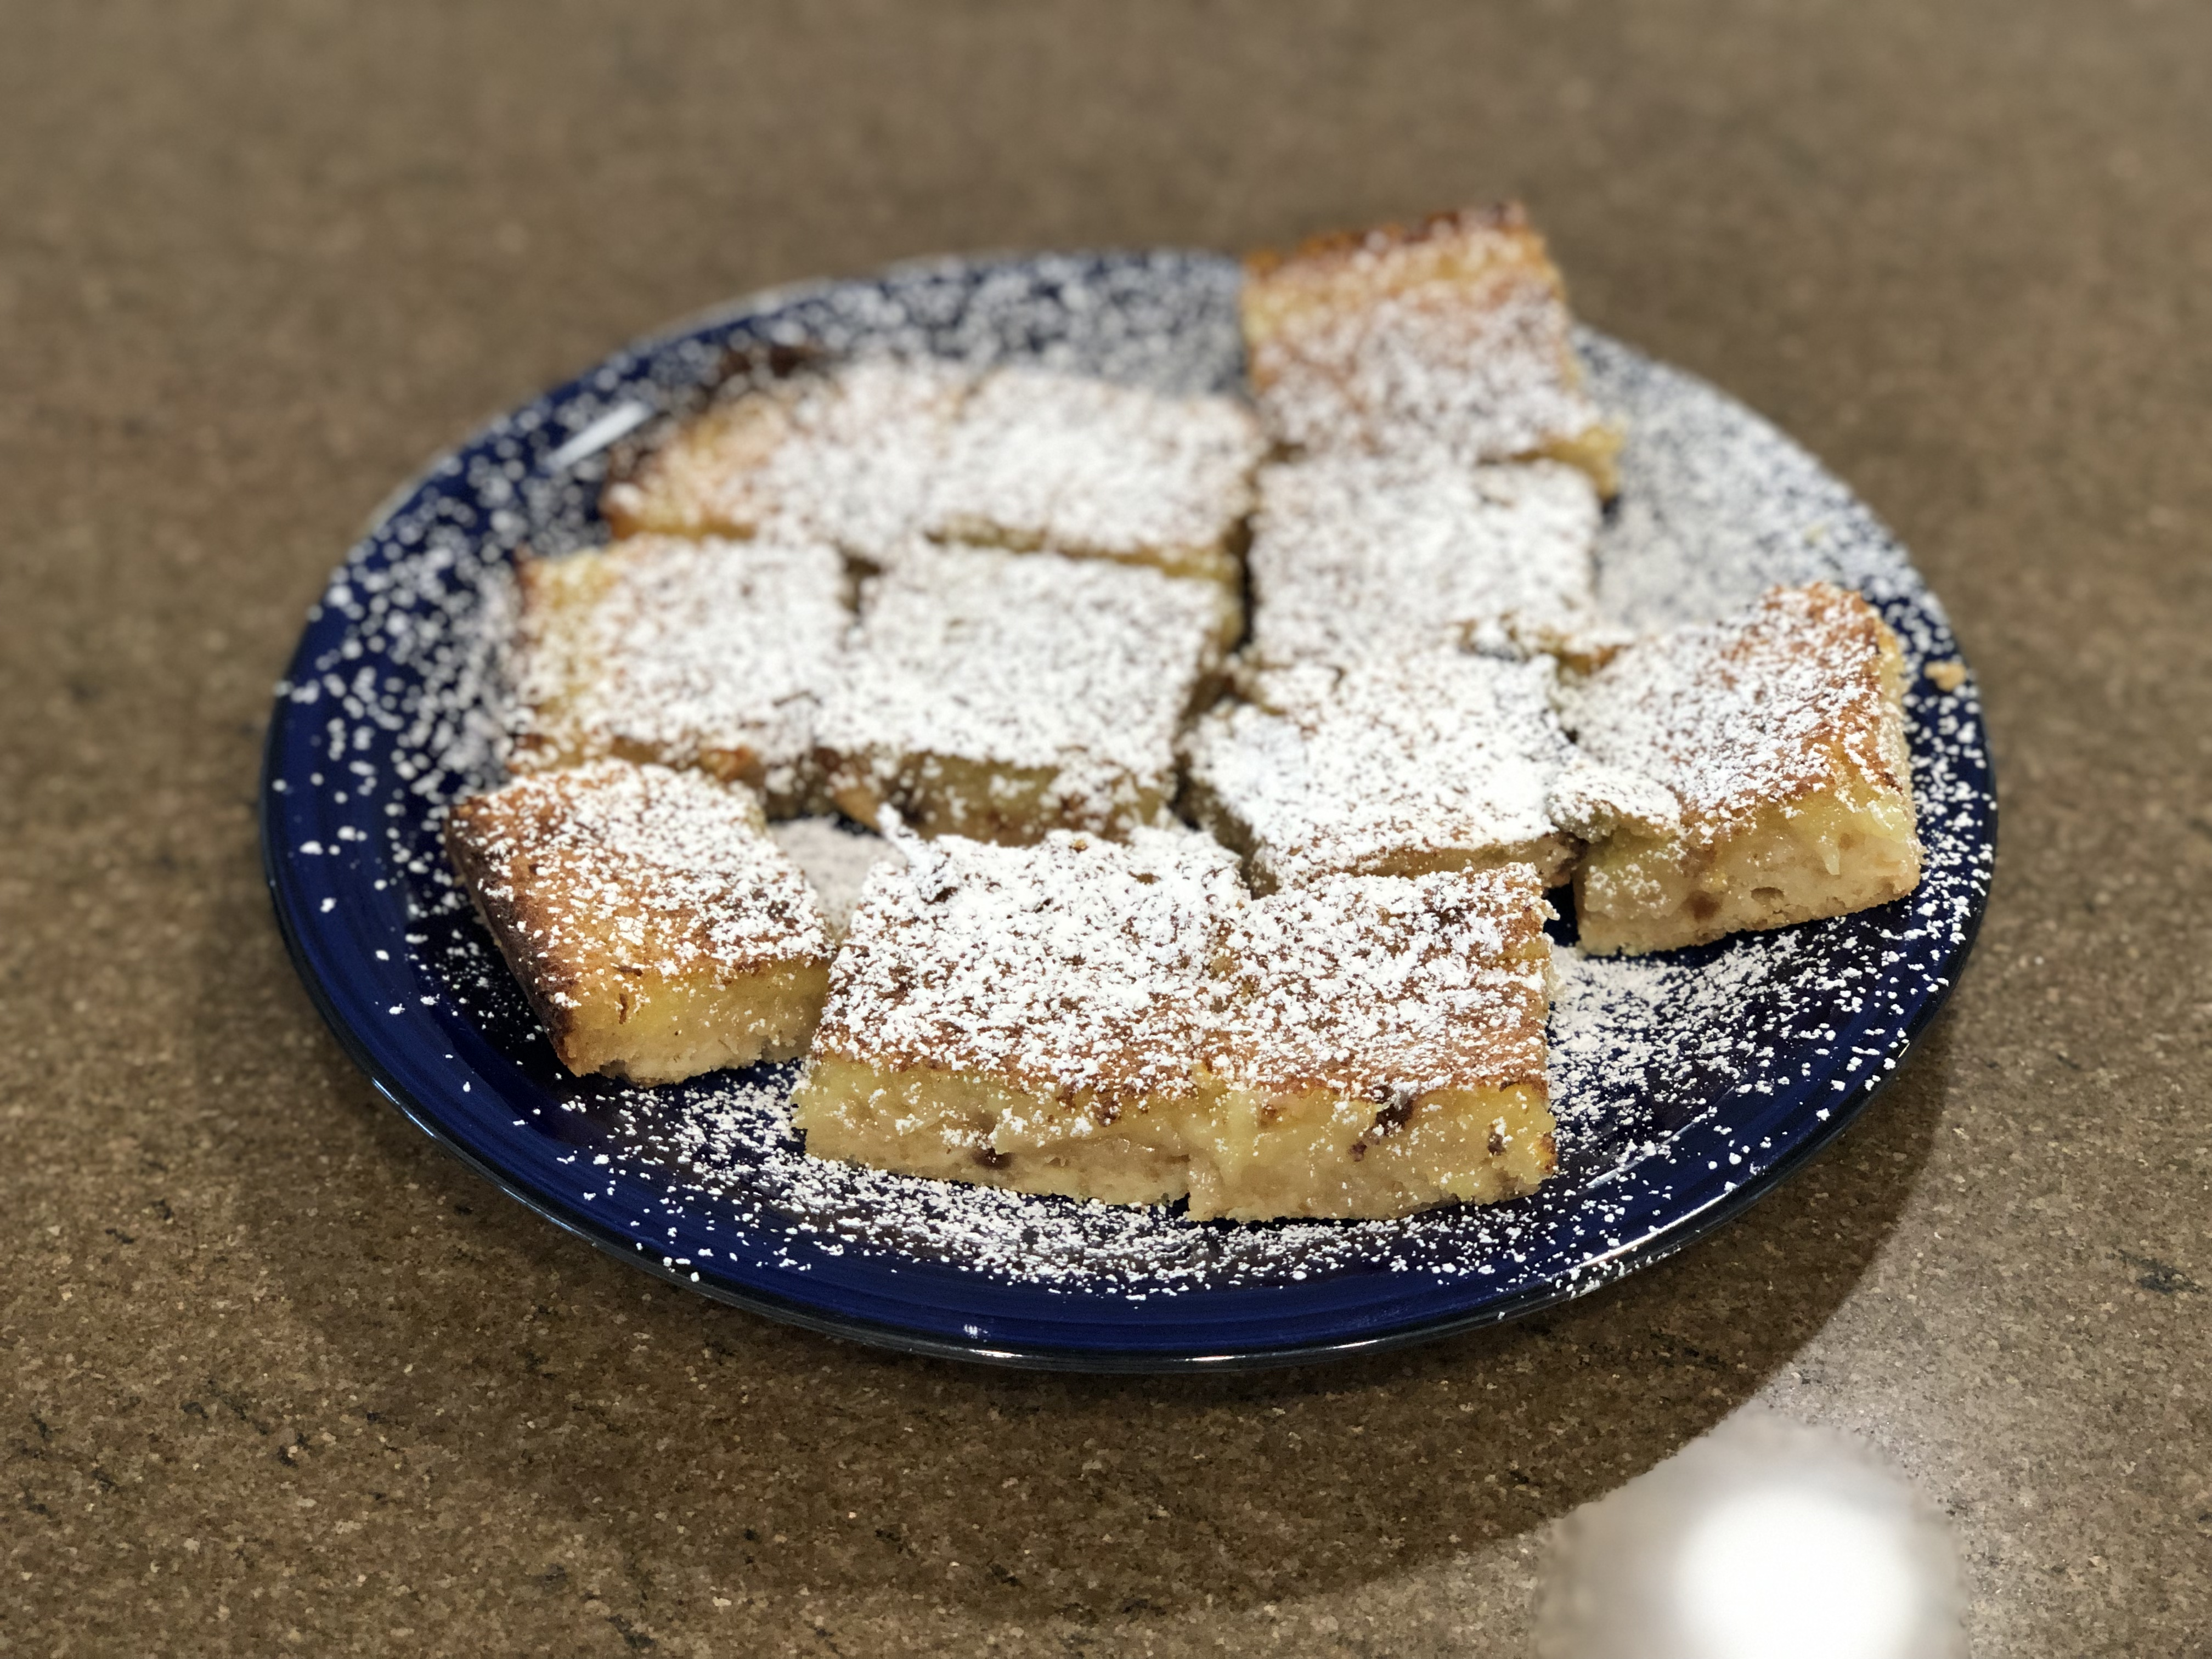
\includegraphics[scale=0.095]{lemon-bar.png}
\end{figure}

\bigskip

\textbf{Ingredients}

\begin{multicols}{2}

    \begin{itemize}
        \item 2 cups flour
        \item 1 cup (2 sticks) butter, softened
        \item \sfrac{1}{2} cup powdered sugar
        \item \sfrac{1}{2} teaspoon salt
        \item 1 tablespoon light brown sugar
        \item 1 tablespoon lemon zest

              \columnbreak

        \item 4 eggs, plus one egg yolk
        \item 2 cups granulated sugar
        \item \sfrac{1}{4} teaspoon salt
        \item 2 - 3 tablespoons lemon zest
        \item 1 teaspoon baking powder
        \item 7 tablespoons lemon juice
    \end{itemize}

\end{multicols}

\textbf{Directions}

1. Spray a $9\times13$ glass baking dish with Pam and set aside.

2. Mix the flour, powdered sugar, \sfrac{1}{2} teaspoon salt, and light brown sugar
with a whisk. Cut the butter into the flour if it's still cool. Or, if you've melted
the butter, just stir it in. Stir in the 1 tablespoon lemon zest. Press this mixture
into the bottom of the baking dish and bake at 350 degrees for 20 minutes.

3. While the crust is baking, combine the remaining ingredients in a medium bowl until
well blended. You can use a whisk or an electric beater. Both work great.

4. When the crust finished immediately remove it from the oven and pour the egg mixture
directly on top. Put this back in the 350 degree oven and bake for 15 to 20 minutes. Don't
worry, it'll get brown spots on top in some spots. This is ok.

5. Remove from oven and let the bars cool completely (yes Mom, completely). Then cut into
$2\times3$'' pieces, move to a plate (this is the hard part, they're sticky), then dust
with some more powdered sugar until they're white and pretty.

\end{document}
